\chapter{Understanding The Behaviour of Retweeting in Twitter}


It is clear how the popularity of a Tweet can be related to its propagation characteristics as it travels through Twitter's social structure. That is to say, that the greater the number of times a Tweet is retweeted by users, the more people have found its contents to be interesting enough to be worth sharing.

It has also been shown that this retweet count metric alone cannot be a direct implication of the actual interestingness level of a Tweet. Reasoning for this is related to the notion of user influence, which dictates that some Tweets are naturally immediately available to more people and thus have a higher chance of achieving a retweet. Indeed, \citet{suh10} demonstrated that a user's Tweets' retweet rates increase as the user's follower count increases.

The strength of Twitter lies in its social structure, where users can elect to follow and unfollow others as they desire and with immediate effect. Followers of a user receive all of that user's posts onto their individual (or `home') timelines. As a result, people are likely to follow users who create more `interesting' posts; whether the follower is very interested in the friend his/herself, or if the follower is simply interested in the topical area of most of the friend's posts. 

Just as Twitter users will post Tweets with subjects that are of interest to them - possibly related to the user's work, a hobby, or a mixture of multiple areas - and these Tweets are generally posted with the idea that they will be useful or interesting for some of their followers as well as an attempt to attract more followers, retweets are generated with the same motives in mind. This means that if a Tweet is retweeted, it is not only allowed to disseminate further through the social structure, but also that a higher Tweet quality is implied.

Thus, this describes how a user's friends, who carry out most of the retweets of the user, effectively become filters of interesting information for that user and for the followers of those friends. The \textit{audience} of the original Tweet is therefore significantly increased. Since retweets are usually always attributed to the original author then you, a Twitter user, may gain more attention by means of followers by posting \textit{interesting} Tweets, which will; 
\begin{enumerate}
\item increase the chances that users reading your Tweets will choose to follow you, and;
\item increase the chances that users will decide to retweet your Tweet, thus broadcasting it to a larger audience. People viewing this \textit{retweet} may then decide to follow you. 
\end{enumerate}

Since a Tweet can be retweeted multiple times, and that a retweet itself can also be retweeted, the much larger the effective audience (both directly and through retweets) of a Tweet's original author has the potential to become if they choose to post interesting information. In this chapter, an understanding of the behaviours and properties of retweets is provided, along with discussions into how these are relevant in researching useful metrics for determining which retweeted information is interesting.

The notion of `global interest' is used in this thesis as a definition of interestingness. Although it is not feasible to say that a particular Tweet is unanimously interesting, it is possible to identify Tweets that are \textit{generally} more outstanding than noise. 

In this chapter, several contributions are made. Key terms, such as retweet group and path-length, are defined in the context of Twitter and Tweet propagation and become a model for much of the remaining work in the thesis; an in-depth analysis into retweet behaviour, including the dynamics of Tweet spread, audience, and temporal characteristics, is made; and discussions are conducted over the penetration of retweets and their relationships to communities on the social graph. Questions \textbf{RQ1} and \textbf{RQ2} from Section \ref{section:research_questions} are addressed, reinforcing the need for the non-semantic inference of globally interesting information.


\section{Tweet and Retweet Properties}
In this section, a more formal overview on retweet properties is provided in addition to an introduction and definition of concepts frequently referred to in the thesis.

\subsection{Retweet Groups}
A Tweet has various attributes associated with it, which make up the features that describe it and its author. These properties relate to the content, the author, and other metadata, such as its creation time, geographical location coordinates, language, and so on. However, not all of these properties are relevant to this research and, as such, a particular Tweet, $t$, has its relevant properties declared and defined as follows;
\[
	t = (\mathrm{text}, \mathrm{count}_R, \mathrm{author}_O, \mathrm{author}_R, \mathrm{orig}, \mathrm{prev})
\]

Respectively, this represents the Tweet's text, its retweet count, and the \textit{original} author of the Tweet. The final three values depend on whether $t$ is a retweet or not and represent the author/forwarder of the retweet, a reference to the original Tweet, and a reference to the \textit{previous} Tweet in the chain respectively, and are all \texttt{null} when $t$ is not a retweet. Since a retweet is simply an extension of a class of Tweet, then the same properties can be assigned to retweets as to Tweets, except that in the case of retweets the values $\mathrm{prev}$, $\mathrm{orig}$ and $\mathrm{author}_R$ will be non-\texttt{null}.

For example, let the Tweet shown in Figure \ref{fig:retweet_button} be $t_1$. This is an original Tweet and has the following properties; 
\begin{flalign*}
t_1.\mathrm{prev} & = \textrm{\texttt{null}}\\
t_1.\mathrm{orig} & = \textrm{\texttt{null}}\\
\aut{t_1}{R} & = \textrm{\texttt{null}}\\
\aut{t_1}{O} & = \textrm{\texttt{Adrian Bradley}}\\
\rc{t_1} & = 0 \textrm{ (at time of writing)}
\end{flalign*}

Inversely, the Tweet displayed in Figure \ref{fig:northern_lights_tweet} ($r_1$) \textit{is} a retweet of another Tweet, $t_2$, where;
\begin{flalign*}
r_1.\mathrm{prev} & = t_2 \quad \textrm{(assumed)}\\
r_1.\mathrm{orig} & = t_2\\
\aut{r_1}{R} & = \textrm{\texttt{Discover The World}}\\
\aut{r_1}{O} & =  \textrm{\texttt{Alda Sigmundsd\'{o}ttir}}\\
\rc{t_2} & = 48 \textrm{ (at time of writing)}
\end{flalign*}
and $\rc{r_1}$ is unknown. $r_1.\mathrm{prev}$ is assumed since $r_1$ was created using the button retweet method, which does not cite any intermediate retweeters, even if they exist.

A Twitter user, $u$, is represented by a Twitter account, and also has a set of properties. In relevance to the work in this thesis, these largely relate to the user's position in the social graph. 

The full social graph, denoted by $G$, comprises $V(G)$, the nodes representing the set of users on Twitter; and $E(G)$, which is the set of edges connecting these nodes. In Twitter's case, the edges denote the followships between users, and are therefore \textit{directional}. Thus, the set of followers and the set of friends of user $u \in V(G)$ are denoted by $\fos{u}$ and $\frs{u}$ respectively, where;
\[
    \fos{u} = \left\{u \in V(G) :  \overrightarrow{u v} \in E(G)\right\}
    %\quad \forall \quad 0 \leq i \leq |G| \quad : \quad \exists \quad \overrightarrow{u_i u} \right\}
\]
\[
    \frs{u} = \left\{u \in V(G) :  \overleftarrow{u v} \in E(G)\right\}
    %\left\{u_i \quad \forall \quad 0 \leq i \leq |G| \quad : \quad \exists \quad \overleftarrow{u_i u} \right\}
\]
In other friendship-based social networks, such as Facebook, relationships are mutual and are therefore represented by non-directional edges in the relevant social graphs.

The terms $\foc{u}$ and $\frc{u}$ respectively refer to the in-degree and out-degree of a user $u$, where $u \in V(G)$. These in turn represent the cardinality of each of the sets of followers and friends of $u$, and therefore the author of Tweet $t$ has a follower count of $\foc{\aut{t}{O}}$ and a friend count of $\frc{\aut{t}{O}}$.

Let $T$ represent the set of \textit{all} Tweets. Since a Tweet can be retweeted more than once, and have its retweets also retweeted, the set of retweets of Tweet $t \in T$ is defined as;
\[
    \rt{t} = \left\{ r \in T : r.\textrm{orig} = t \right\}
\]

Hence, the retweet count of $t$ is given by $ \rc{t} = \left\vert{\rt{t}}\right\vert $.


\begin{mydefinition}
\label{definition:retweet_group}
A \textbf{retweet group}, denoted by $\rg{t}$, describes the original Tweet, $t$, along with the set of the retweets of $t$, $\rt{t}$. Thus;
\[
    \rg{t} = \left\{t\right\} \cup \rt{t}
\]
\end{mydefinition}


Retweet groups are useful for identifying a Tweet and the retweet replicas of it, and is appropriate when discussing the audience reach of a particular Tweet. Therefore, since $t$ is also a member of this set, the size of $t$'s retweet group is; 
\[
	\left\vert{
\rg{t}}\right\vert = \rc{t} + 1 
\] 
which can have a minimum cardinality of one - $\rg{t} = \left\{t\right\}$ - in cases when not retweeted at all.
 

\subsection{Retweet Trees}
As a Tweet gains popularity and is retweeted more, and since its retweets themselves can \textit{also} be retweeted, then this results in the generation of a retweet \textit{tree}, which represents the retweet group of a particular Tweet. This tree illustrates the original Tweet and the various propagation pathways it takes as it is retweeted through the social graph. 

The tree is not a representation of the actual social ties between the authors of the tree's nodes, as users are able to retweet Tweets and retweets sent from others that they do not follow. However, as is mentioned later in this chapter, most retweeting does generally occur between directly-linked users. \cite{kwak10} also uses retweet trees to assist in illustrating information dissemination in Twitter, particularly in observing the Twitter reactions to the 2009 Air France airline crash.

The root of the tree is $t$ and, if $t$ has been retweeted, each of the other nodes are made up of the set of retweets in $\rt{t}$. Each non-root member of the tree refers to its parent through its own `$\textrm{prev}$' attribute, as illustrated in Figure \ref{fig:retweet_tree}. Retweet trees are useful for this purpose as they help demonstrate the temporal `paths' down which the retweets occur and the chains they produce. A similar illustrative device is used by \citet{galuba10} in describing URL cascades in Twitter.

\begin{figure}[h]
\centering
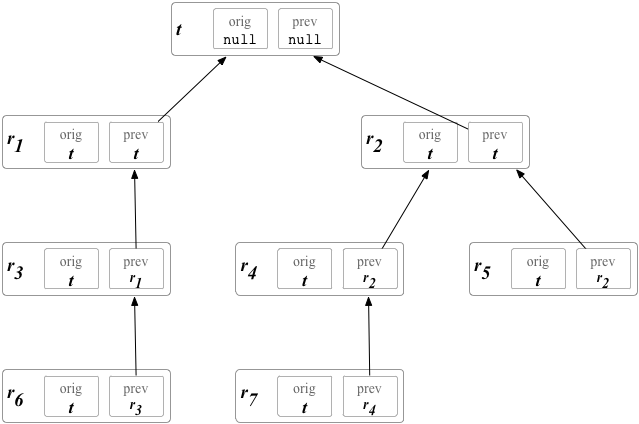
\includegraphics[scale=0.6]{3.Chapter1/Media/tree.png} 
\caption{A hypothetical retweet tree.}
\label{fig:retweet_tree}
\end{figure}

In very rare cases, more than one node in a retweet tree may share an author user. This only occurs when a particular user retweets a Tweet more than once, and would only generally happen in scenarios where the user is using the manual method to modify the content as part of a conversation with others or for expressing multiple opinions. For example, a user may receive a Tweet relating to a particular news story, and then decide to retweet it with a small annotation. Upon feedback from followers, the user then retweets the Tweet again, yet with a different annotation. Each of these new retweets could then become the root of two branches in the complete tree of the Tweet.

Retweeting the same Tweet multiple times is not supported through the button method. Once a Tweet has been retweeted by a user in this way, there is no provision for the functionality to retweet a different member of the same group or, indeed, the original Tweet. A retweet can be `un-done' by clicking the button again on any member of the retweet group, yet this will not affect further retweets of this retweet that have been made using the button method.


\subsection{Path-Length}
In addition to retweet groups having a size property, a retweet groups's branch's \textit{path-length} refers to the length of a particular retweet chain. 

\begin{mydefinition}
\label{definition:path_length}
The \textbf{path-length} of a single retweet chain in a retweet group is defined as the number of hops between a Tweet, $t$, and the retweet represented by the leaf node of the chain's branch in $\rg{t}$'s tree.\\
The \textbf{maximum path-length} of a retweet group is the greatest path-length observed in the retweet group.
\end{mydefinition}

Figure \ref{fig:retweet_tree} represents the members of the retweet group of a hypothetical Tweet, $t$. This retweet group has a size of 8 and has 3 distinct retweet chains, the longest of which are the two involving [$t, r_1, r_3, r_6$] and [$t, r_2, r_4, r_7$]. The \textit{maximum} path-length of this retweet group is therefore 3, as the leaf node of both of these branches is three hops away from the original Tweet at the root.

Although the tree does not illustrate the edges between users on the social graph, it is possible for the underlying graph to connect the authors of the tree's nodes in various ways. For example, it is likely that $\aut{r_3}{R}$ follows $\aut{r_1}{R}$, but it's also possible that $\aut{r_3}{R}$ follows $\aut{r_2}{R}$. More on this topic is discussed in the audience analysis in Section \ref{section:audience} and in the social graph analyses in Section  \ref{section:retweets_graph}.

When a user retweets a Tweet or retweet through the manual approach, the current test of the Tweet is pre-pended with the sequence \texttt{RT @<username>:}. Therefore, a Tweet with the content;\newline
\texttt{RT @user2: RT @user1: This is the body of the Tweet}\newline
was originally authored by \texttt{user1}, then retweeted by \texttt{user2}, and then finally retweeted by the author of this current retweet (a Tweet or retweet's author's username is not credited in the body of the text in this way). Making such citations does count towards the 140 character Tweet limit, which may partially explain the path-length distribution pattern observed later in Section \ref{section:pathlength}.

It should be noted that this phenomenon can only be observed through retweets by the manual approach, since the button method always simply credits the original author, and not any of the internal members of the retweet group. Although a significant number of retweets today are carried out using the button method, the manual approach still remains popular currently and even more so at the time the research in this chapter was carried out in the spring of 2011. This allowed for making useful observations of retweet patterns that could not be as successful later on.


\section{Information Searching and Affective Stimulation}
A Twitter user electing to follow another user cannot, in most cases, predict precisely what the new friend will Tweet about in the future. The user has some \textit{expectation} of the type of information they are likely to receive based on the previous Tweets of the new friend, which is generally the main cue the user can use to base the follow decision on.

Part of the follow decision is based on the notion of relevance judgement, which is an idea discussed at more length by \citet{xu07} and is partly made up of the goal of achieving \textit{affective stimulation} through \textit{hedonic} searching as opposed to the use of \textit{epistemic} searching.

\subsection{Epistemic Search}
An epistemic information search is one that involves carrying out a search with the purpose of finding out information on a particular topic (or set of) to satisfy a \textit{desire for knowledge} \cite{xu07}, yet without an actual aim to solve any particular problem.

An example of this type of search is a `crawl' through Wikipedia, in which a searcher may start at one particular page of interest and then follow links within that page to other related pages of interest that stem away from the source topic. In this case, the search `parameter' is simply the name or title of the article the searcher wants to view. As mentioned previously, a followship between users is effectively a search parameter in Twitter, since the following user has elected to follow the new friend to receive information from him/her. It is clear that this type of `searching' cannot be epistemic as the following user cannot know exactly the \textit{type} of information they are going to receive.

\subsection{Hedonic Search and Affective Stimulation}
\label{section:affective_stimulation}
Hedonic searching is similar to epistemic searching in that it is also not carried out with the aim to solve an immediate problem, but is different in that it is done to search for fun or `affective stimulation' \cite{xu07}.

A person can be said to be affectively stimulated if he/she views a piece of information that has some effect on the person, such as something that conveys emotion, something that is of particular interest to the person, or something that is capable of provoking some further thought.

With hedonic searching, users are not aware of the information that they are going to receive prior to searching and thus cannot really predict any level of affective stimulation. This aligns more with Twitter usage, since users receive information that they cannot accurately foresee. Any Tweets received that do provide interesting information can convey affective stimulation to the user. This is the type of information that becomes harder to identify amongst lots of noise, yet is also the type of information a user is more likely to retweet.


\subsection{The Recognition Heuristic} 
A further metric for measuring information relevance in information retrieval is the recognition heuristic. This heuristic takes advantage of a person's memory and declares that if a person is able to recognise only one of two (or more) items, then s/he is more likely to judge the recognised item to be `greater' or more important \cite{oppenheimer03, goldstein99}.

Relating this to information received on Twitter, \citet{chorley12} found that a user recognising a Tweet's author significantly increases the chance that the user will decide to read the Tweet. Since a user must read a Tweet in order to make a decision on whether, or not, to retweet it, then the recognition heuristic transiently plays a part in a user's retweet decision also.

The authors also find that information about the Tweet itself, such as its text content and its retweet count, has much more of an effect on a user's read decision than information about the author, such as the followers count or Tweet rate. This also contributes to the declaration that information interest goes beyond the features surrounding a particular user and that user influence does not dictate interestingness of information.


\section{Twitter Propagation Analysis}
Understanding information propagation in Twitter is key to also understanding how interesting information might be detected. Whilst it is known that the retweet count of a Tweet cannot be used alone in inferring interestingness, since this is simply a level of popularity tied in with the author user's influence, it is still a factor in that users are more likely to retweet interesting information than noise.

Of particular interest is to achieve an overview of propagation behaviours in Twitter; the patterns in the properties of retweet groups, such as their sizes and penetration depth, temporal aspects of retweets and information on the social structure of Twitter itself with regards to propagation within it.

The remainder of this chapter involves an exploratory study of the retweet characteristics in Twitter to provide a further background, and which demonstrates the area's relevance towards the goal of inferring interesting information.


\section{Retweet and Retweet Group Analysis}
To assist in providing a further grounding in this area of research, a series of analyses were carried out into retweets and retweet groups. This section describes the processes and purposes of the analyses.


\subsection{Data Collection Methodology}
The analyses involve the examination of Tweets extracted from Twitter's REST API v1, which was used between 26\textsuperscript{th} January and 24\textsuperscript{th} May 2011 to collect Tweets and retweets from the public timeline.

The data collection involved a mixture of using Twitter's timelines and its search capabilities. Version 1 of the REST API supported retrieval of Tweets, 20 at a time, from the Twitter \textit{public} timeline. Historically, this timeline contained the 20 most recent Tweets published by all the authors that have non-protected Twitter accounts, and it used to be visible on their website's homepage\footnote{http://twitter.com} to non-logged-in users.

In particular, for the data-collection periods, the public timeline endpoint was queried every ten seconds to retrieve the current set of the most recent public Tweets. Millions of Tweets are posted each hour, and ten seconds was a granular-enough frequency to ensure that there was no duplication in the data returned. From all of the retrieved Tweets, the ones that were retweets were filtered out and stored. Retweets, as mentioned earlier, are distinguishable since they start with the characters `RT' followed by a username. It should be noted that when retrieving Tweets from Twitter's API that even retweets that were created using the button method begin with the same character sequence, allowing detection of these also.

Following storage, the content of the retweets were parsed in order to extract the text that the original Tweet contained. Sometimes, retweets using the manual approach are used to provide additional annotation to the Tweet. Although this can often be distinguished by the fact that the original Tweet content is inside quotation marks (`` ''), it is not true in all cases, meaning that sometimes the original text could not be reliably extracted programmatically by a machine. In these cases additional queries were made to Twitter's search API in an attempt to resolve the problem, yet, failing that, the retweet was discarded.

Once the original text had been successfully extracted, this was used along with other metadata as query parameters to Twitter's search API in order to try and find the original Tweet and any other retweets of this Tweet. The search API uses approximate (or `fuzzy') string matching, but quotation marks can be used to retrieve search results based on an exact string pattern\footnote{https://dev.twitter.com/docs/using-search}.

Once the API search was complete (in some cases, with Tweets achieving many retweets, many API calls were required in order to page through results), the original Tweet could easily be identified as the only one of the set \textit{not} starting with the sequence ``RT''. This provided a retweet group comprising the original Tweet and all available retweets of this Tweet.

On some occasions, more than one Tweet were each identified as the original Tweet and so no data was stored for this group. This could occur, for example, if many users Tweet exactly the same text coming from an external source, such as a news webpage, and means that the entire set of retrieved Tweets are not likely to be part of the same retweet group. In cases where no results were returned, the retweet was not stored and was assumed to be an orphan retweet, perhaps as a result of a retweet of a Tweet posted by a protected Twitter account. Where no original Tweet could be identified it was sometimes possible to identify it through cross-matching against other retweets in the retrieved retweet group, but were discarded if unsuccessful.

The retweet groups were finally stored along with relevant metadata in order to carry out the studies described in the following sections. The data consisted of a set of around 4,400 retweet groups, which comprised of 26,000 Tweets (defined as $T'$)  and retweets. The relatively limited size of the dataset is acknowledged, yet it should be emphasised that these analyses are simply exploratory and are not used to answer or solve any specific problem.


\subsection{Exploring Retweet Group Path-Lengths}
\label{section:pathlength}
The path-lengths of each chain in a retweet group can be calculated by identifying the members involved in retweet activity down that chain; from the original Tweet to the final retweet. The \textit{maximum} path-length of a particular retweet group is the longest path-length observed in the group's tree.

Identification of path-lengths can be carried out through parsing the text of a retweet, and following the citations. Although it cannot be guaranteed that all users will be properly cited in a chain, and there is no realistic method to verify this, it is felt that correct citations will be made enough times to make these cases relatively insignificant.

On average, the maximum path-length observed across the retweet groups was around 1.8, with the vast majority of retweet chains being between one and two edges in length. When one considers that many retweets are made through the button method, which removes citations of internal users in the chain and simply credits the original author and would therefore produce many single-length retweet chains, this average will theoretically be an underestimate. The similar observations made by \citet{kwak10} in the area also indicate a large number of groups with maximum path-lengths of one and two.

The longest observed maximum path-length was nine, which is a huge depth of penetration through the social structure since the total number of users involved in propagating the Tweet was ten. This, combined with the knowledge that social networks can represent a `closer' social graph than the real world's six degrees of separation, shows how retweeting can have a huge impact in information spread amongst millions of people worldwide very quickly. Figure \ref{fig:pathlength-distribution} illustrates the distribution of maximum path-lengths observed in the retweet groups of Tweets in $T'$.

\begin{myobservation}
\label{observation:path-length}
The mean maximum path-length observed across the retweet groups analysed was around 1.8.\\
The longest maximum path-length observed was 9.
\end{myobservation}

\begin{figure}[h]
\centering
    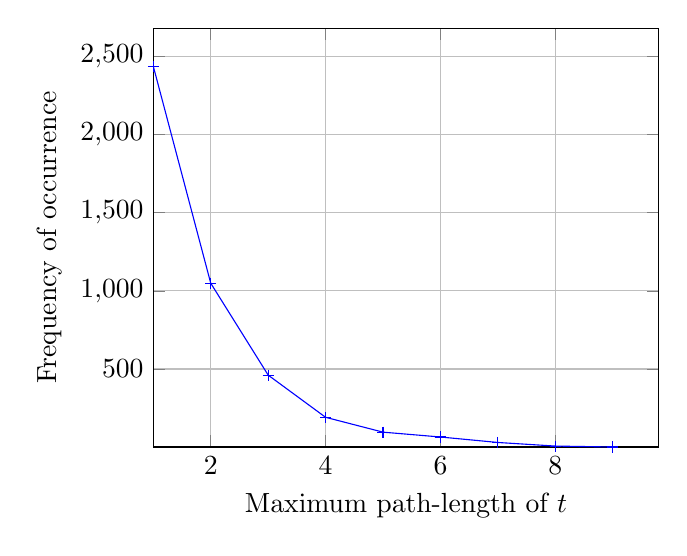
\begin{tikzpicture}
     \begin{axis}[
            xlabel=Maximum path-length of $\rg{t}$,
            ylabel=Frequency of occurrence,
            grid = major,
            width=8cm,
            xmin = 1,
            ymin = 1
            ]
        \addplot[mark=+,blue] plot coordinates {
            (1,2437) (2, 1049) (3, 461) (4, 191) (5,96) (6,65) (7,30) (8,7) (9,1)
            };
            % Data from pathlength-distribution.csv
    \end{axis}
    \end{tikzpicture}
    \caption{Distribution of maximum path-lengths observed in $\rg{t} \, \forall \, t \in T'$.}
    \label{fig:pathlength-distribution}
\end{figure}

Also of interest is the relationship in terms of the social ties between the different authors of the Tweets in a retweet group. In cases where a retweet group's maximum path-length is precisely one, i.e. the situation where a user (or set of) has retweeted a particular Tweet only once, the retweeting authors of the leaf Tweets of this group's retweet tree follow the original author around 90\% of the time.

This implies, therefore, that in the remaining 10\% of cases, a retweeter has retweeted a Tweet from outside of their home timeline and has instead seen a Tweet whilst browsing through another user, who isn't a friend, timeline that the retweeter regards as sufficiently interesting. This helps to demonstrate that the more followers a particular user has, the greater the chance that another user somewhere has of viewing the user's Tweets and then having the opportunity to retweet them. The fact that 90\% of retweets of a particular user are created by direct followers reinforces this further.

This particular property could also be partly due to use of the button method of retweeting, which does not cite intermediate retweeters, and thus always imply that the final retweeter directly retweeted the Tweet from the original author. However, there may, in fact, have been other retweeters in between the final retweeters and original author, each of which following the immediately upstream retweeter. As such, this 90\% follow probability between the retweeter and source user in 1-hop retweet chains is also likely to be an underestimate.

%\begin{figure}[h]
%\centering
%    \begin{tikzpicture}
%    \begin{axis}[
%        symbolic x coords={1,2,3,4,5,6},
%            ylabel=Likelihood of citation of $\aut{t}{O}$,
%            xlabel=Maximum path-length of $\rg{t}$,
%            ymin=0,
%            ymax=100,
%            ybar,
%            bar width=7pt
%            ]
%       \addplot plot coordinates{
%            (1,72) (2,64) (3,60) (4,64) (5,65.5) (6, 83.5)    
%        };    
%    \end{axis}
%    \end{tikzpicture}
%    \caption{Proportion of cases where the original author is cited with varying maximum path-length of retweet group}
%\label{fig:citation-pathlength}
%\end{figure}

Further to this, in situations in which the maximum path-length of a retweet group is \textit{greater} than one, retweeting authors in the group follow the author of the original Tweet about 40\% of the time. It is clear from Figure \ref{fig:totalretweets-pathlength} that retweet groups with a longer maximum path-length tend to have a larger size themselves. This increases the likelihood that the Tweet has been able to spread both further around the original Tweet's author's community, and also the potential for the Tweet to `travel' to other communities. Since users from outside the source user's community are less likely to follow the source user, this explains the reduction in the followship likelihood between further downstream retweeters in the retweet chains and the original author.


\subsection{Size of Retweet Groups}
The distribution of retweet group sizes $\, \forall \, t \in T'$  was found to follow a power-law type distribution, with a relatively large $p$-value of around $0.87$. Figure \ref{fig:retweet-distribution} represents the complementary distribution function demonstrating the changing probability of a randomly generated $X$ being greater than or equal to $x$, the `current' value of $|\rg{t}|$, at each stage. The techniques used in this analysis are adapted from the methods and code provided by \citet{clauset07}.

\begin{figure}[h]
\centering
    \begin{tikzpicture}
     \begin{loglogaxis}[
            xlabel=$x$,
            ylabel=$P(X \geq x)$,
            grid = major,
            width=8cm,
            ]
        \addplot[mark=+,blue, only marks] plot coordinates {
(1,1) (2,0.6) (3,0.45) (4,0.4) (5,0.31) (6,0.29) (7,0.26) (10,0.21) (15,0.20) (16,0.19) (17,0.16) (18,0.145) (19,0.14) (20,0.13) (31,0.125) (32,0.118) (33,0.10) (39,0.09) (57,0.077) (82,0.068) (157,0.044) (310,0.035) (700,0.025) (1100,0.012)
            };
        \addplot[mark=none,red] table[mark=none,blue,row sep=\\,
            y={create col/linear regression={y=Y}}]{
            X Y\\
            1 1\\
            2 0.6\\
            3 0.45\\
            4 4\\
            5 0.31\\
            6 0.29\\
            7 0.26\\
            10 0.21\\
            15 0.20\\
            16 0.19\\
            17 0.16\\
            18 0.145\\
            19 0.14\\
            20 0.13\\
            31 0.125\\
            32 0.118\\
            33 0.10\\
            39 0.09\\
            57 0.077\\
            82 0.068\\
            157 0.044\\
            310 0.035\\
            700 0.025\\
            1100 0.012\\
        };
            % Data from pathlength-distribution.csv
    \end{loglogaxis}
    \end{tikzpicture}
    \caption{Maximum likelihood power-law fit for the cumulative distribution of retweet group sizes}
    \label{fig:retweet-distribution}
\end{figure}

The mean group size from this dataset was found to be just below six, and the largest size was 284. The smallest $|\rg{t}|$ were the cases in which $\rc{t} = 1$, and which were significantly the most common occurrences.

\begin{myobservation}
The mean observed retweet group in the dataset $T'$ was of size 6.
\end{myobservation}

Of interest also is the relationship between a group's size and its maximum path-length. Generally, the maximum path-length of a group, $\rg{t}$, increases with $|\rg{t}|$, indicating a mostly uniform growth in the retweet trees representing these groups - as might be expected. Figure \ref{fig:totalretweets-pathlength} demonstrates this trend, which illustrates that as the retweet count of $t$ increases, then the longer the retweet chains in $\rg{t}$ are likely to become. This would increase its penetrative dissemination away from the source and further facilitate its spread between communities, increasing its potential \textit{audience size}.

\begin{figure}[h]
\centering
    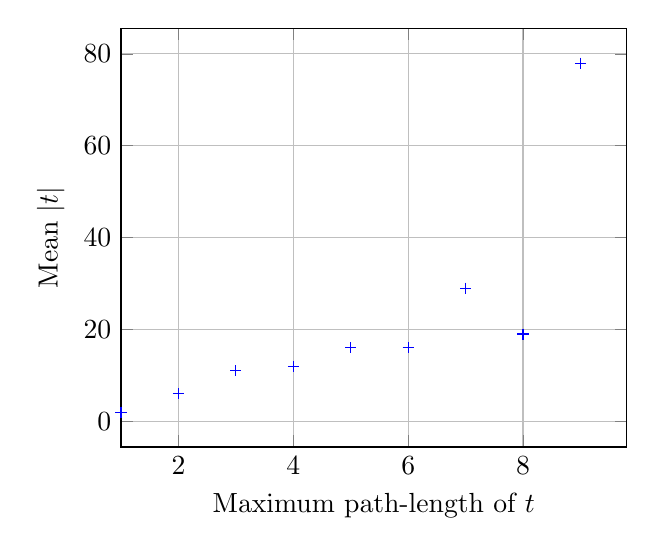
\begin{tikzpicture}
    \begin{axis}[
            ylabel=Mean $|\rg{t}|$,
            xlabel=Maximum path-length of $\rg{t}$,
            grid=major,
            xmin=1,
            width=8cm]
       \addplot[mark=+,only marks,blue] plot coordinates{
            (1,2) (2,6) (3,11) (4,12) (5,16) (6, 16) (7,29) (8,19) (9,78)    
        };    
    \end{axis}
    \end{tikzpicture}
    \caption{Relationship between the maximum path-length and size of a retweet group. The greatest path-length was included for context, but had a sample size of only one}
\label{fig:totalretweets-pathlength}
\end{figure}

\subsection{A Tweet's Audience - How Many Users Can be Reached?}
\label{section:audience}
$\rg{t}$'s (immediate) audience size refers to the number of Twitter users that have received $t$, either in its original form or as a retweet, $r$, such that $r.\textrm{orig} = t$. Users in the audience are not guaranteed to have read the Tweets, but they are the users who will have received the Tweet on their home timelines.

The term `immediate' is used to signify the distinction between those users who passively receive the Tweet, due to following the original author or a retweeter, and those who see the Tweet whilst actively browsing through other user timelines or the public timeline. Users in the latter group are therefore not direct followers of $\aut{t}{O}$ or $\aut{r}{R} \, \forall \, r \in \rt{t}$ and thus cannot be tracked as members of $t$'s audience.

Let $ r_1,...,r_n $ be the members of $\rt{t}$. The size of the audience of $\rg{t}$ can then be calculated thus (assuming $\rc{t} \geq 1$);
\[
	|\raa{\rg{t}}| = |\fos{\aut{t}{O}}| + |\fos{\aut{t}{r^1}}| + ... + |\fos{\aut{t}{r^n}}| 
\]
where $\aut{t}{r^1} ... \aut{t}{r^n}$ are the users who retweeted $t$.

Despite this, properties of Twitter's social graph dictates that this audience size calculation is na{\"i}ve in that, particularly in the case of more tightly-knit communities, users who are authors of $t$ or $r \in \rt{t}$ are likely to share a subset of each of their followers. The more dense the communities, the more followers are likely to be shared between the authors in $\rg{t}$ and, as such, the aforementioned audience calculation is likely to be an overestimate in nearly all cases. As such, $\raa{\rg{t}}$ is a list and not a formal \textit{set} of users, since it is likely to have some non-distinct members.

The following analyses of retweet group audience sizes relies on a dataset which began collecting at a later date than the general set used in this chapter, and thus the data represented in the rest of this section contains 2860 of the total 4400 groups originally collected. The longest maximum path-length of retweet groups observed in this subset was eight.

The \textit{overhead} of a group, $\rg{t}$, which attempts to address this problem, is related to the level of redundancy of received information by the audience.

\begin{mydefinition}
    $\rg{t}$'s \textbf{overhead} is a value equal to the number of users in $\raa{\rg{t}}$ that receive $t$ or any $r \in \rt{t}$ more than once and, if received more than once, the number of times $t$ is received by each user.
\end{mydefinition}

The audience overhead was found to exist (be greater than 0) in 71\% of all observed retweet groups, further reinforcing that retweets often occur within communities containing users sharing many edges.

Therefore, the actual audience of a Tweet is given by the \textit{set} of users that can be found by modifying the existing definition to take the overhead into account;
\[
	\dia{\rg{t}} = \fos{\aut{t}{O}} \cup \fos{\aut{t}{r^1}} \cup ... \cup \fos{\aut{t}{r^n}}
\]
where $\aut{t}{r^1}, ..., \aut{t}{r^n}$ are the users who retweeted $t$. This definition (`distinct') of audience is used in preference over the previous (`raw') definition for the remainder of the thesis.

 The \textit{proportionate} overhead is defined as the ratio of the overhead to the audience size, and is sometimes more useful for analysing the size of the overhead compared to the popularity of the original Tweet.

For example, a Tweet $t$ has been received onto the home timelines of 800 users as a result of a single retweet, $r_1$. 400 of those users received the Tweet twice due to the presence of shared followers between $\aut{t}{O}$ and $\aut{r_1}{R}$. In this case, the overhead is 400, the proportionate overhead is 0.5, the `raw'  audience has a size of 1200, and the `distinct' audience has a size of 800.

\begin{figure}[h]
\begin{subfigure}{.5\textwidth}
    \centering
    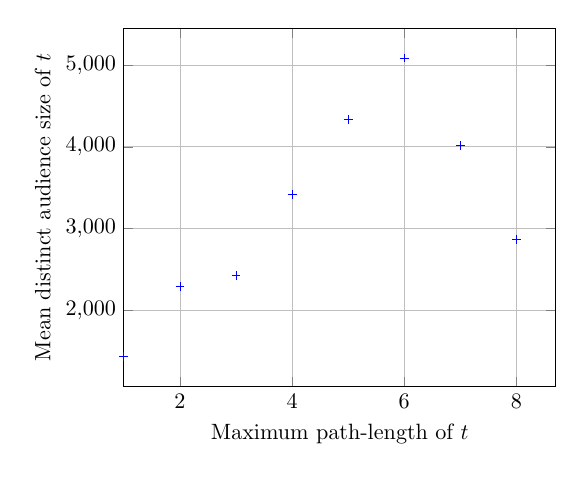
\begin{tikzpicture}[scale=0.8]
    \begin{axis}[
            ylabel=Mean distinct audience size of $\rg{t}$,
            xlabel=Maximum path-length of $\rg{t}$,
            grid=major,
            xmin=1]
       \addplot[mark=+,only marks,blue] plot coordinates{
            (1,1430) (2,2294) (3,2427) (4,3421) (5,4333) (6,5087) (7,4015) (8,2862)
        };    % audienceDISTINCT_pathlength.csv
    \end{axis}
    \end{tikzpicture}
    \caption{Varying $\rg{t}$'s \textit{distinct} audience size with its longest path-length.}
    \label{fig:pathlength-audience}
\end{subfigure}
\quad
\begin{subfigure}{.5\textwidth}
    \centering
    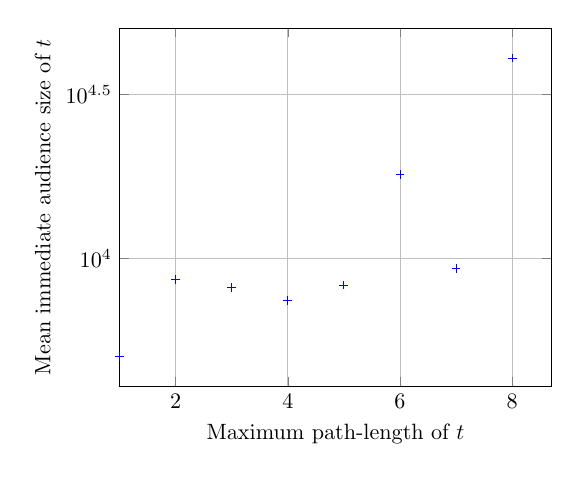
\begin{tikzpicture}[scale=0.8]
    \begin{semilogyaxis}[
            ylabel=Mean immediate  audience size of $\rg{t}$,
            xlabel=Maximum path-length of $\rg{t}$,
            grid=major,
            xmin=1]
       \addplot[mark=+,only marks,blue] plot coordinates{
            (1,5030) (2,8660) (3,8175) (4,7474) (5,8313) (6,17977) (7,9351) (8,40705)
        };    % audienceDISTINCT_pathlength.csv
    \end{semilogyaxis}
    \end{tikzpicture}
    \caption{Varying $\rg{t}$'s \textit{raw} audience size with its longest path-length.}
    \label{fig:pathlength-rawaudience}
\end{subfigure}
\caption{Comparison of the relationships between a $\rg{t}$'s distinct and raw audience size and its maximum path-length $\forall \, t \in T'$}
\label{fig:audience_and_pathlength}
\end{figure}

Figure \ref{fig:audience_and_pathlength}(\subref{fig:pathlength-audience}) illustrates, initially, that which might be expected; that the distinct audience size of a Tweet, $t$, is mostly proportional to the maximum path length of $\rg{t}$. However, as the maximum path-length of retweet groups exceeds 5, then a \textit{decline} in the distinct audience size is observed. This particular behaviour has an unclear cause, but it is felt that this could be related to the saturation of the proportionate overhead's ratio at this stage - in particular, that retweet groups attracting many retweets are circulated more within communities than outside and between communuties. At this stage, the overhead becomes so large, causing this reduction in audience size. This is significant in that the distribution of the non-distict over the increasing path-lengths demonstrates, mostly, a continuous positive correlation (Figure \ref{fig:audience_and_pathlength}(\subref{fig:pathlength-rawaudience})).

 

The \textit{largest} overhead was of a size over six times greater than the group's distinct audience size itself, indicating a massive overlap between the followers of the author of the original Tweet and the authors of its retweets. Whilst the audience overhead was only found to be greater than the distinct audience size in around 3\% of observed retweet groups, it is still clear that the potential for overlap in the followers of retweet group members can be very large in more closely-knit communities Figures \ref{fig:4_overhead}(\subref{fig:pathlength-largestoverhead}) and \ref{fig:4_overhead}(\subref{fig:pathlength-largestproportionateoverhead}) show that the largest overheads observed diminishes in groups with greater maximum path-lengths, which helps illustrate this concept.

Conversely, Figures \ref{fig:4_overhead}(\subref{fig:pathlength-meanoverhead}) and \ref{fig:4_overhead}(\subref{fig:pathlength-meanproportionateoverhead}) respectively show that the \textit{mean} overhead and mean proportionate overhead increase in retweet groups with greater maximum path-lengths. It is assumed that with larger retweet groups there is a greater chance for overlap between the followers of the authors of the members due to there being a greater audience size. Since it is known that increases in the sizes of groups can be indicated by increases in the groups' maximum path-lengths, then this suggests that, on average, the overhead should increase with maximum path-length. 

The diminishing behaviour observed in the other two previously-discussed subplots suggest that these groups with smaller maximum path-lengths exhibiting greater overheads are those that do not fit the trends across retweet group size and maximum path-length observed earlier in this chapter. As such, it is likely that these groups are actually large, with representative trees that are shallow and very \textit{wide}. This illustrates that the Tweets have not propagated far from the original author, yet have circulated thoroughly through a local community. Indeed, three of the largest five overheads in the set of analysed Tweets occur in retweet groups which have a maximum path-length of one. 


\begin{figure}[h]
\begin{subfigure}{.5\textwidth}
    \centering
    \begin{tikzpicture}[scale=0.8]
    \begin{axis}[
            ylabel=Mean overhead of $\rg{t}$,
            xlabel=Maximum path-length of $\rg{t}$,
            grid=major,
            xmin=0
            ]
       \addplot[mark=+,only marks,blue] plot coordinates{
            (1,159) (2,336) (3,532) (4,590) (5,1148) (6,1321) (7,1020) (8,1258)
        };    % overhead-pathlength.csv
        \addplot[mark=none,red] table[mark=none,blue,row sep=\\,
            y={create col/linear regression={y=Y}}]{
            X Y\\
            1 159\\
            2 336\\
            3 532\\
            4 590\\
            5 1148\\
            6 1321\\
            7 1020\\
            8 1258\\
        };
    \end{axis}
    \end{tikzpicture}
    \caption{Varying mean overhead with maximum path-length.}
    \label{fig:pathlength-meanoverhead}
\end{subfigure}
\quad
\begin{subfigure}{.5\textwidth}
    \centering
    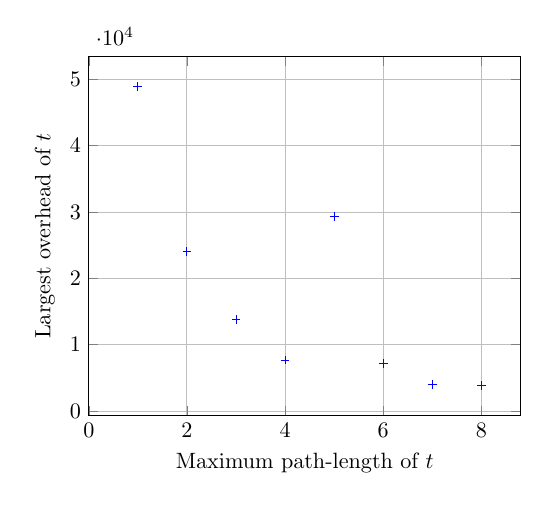
\begin{tikzpicture}[scale=0.8]
    \begin{axis}[
            ylabel=Largest overhead of $\rg{t}$,
            xlabel=Maximum path-length of $\rg{t}$,
            grid=major,
            xmin=0
           ]
       \addplot[mark=+,only marks,blue] plot coordinates{
            (1,48868) (2,23988) (3,13840) (4,7688) (5,29267) (6,7122) (7,3974) (8,3827)
        };    % largestoverhead-pathlength.csv
    \end{axis}
    \end{tikzpicture}
    \caption{Varying \textit{largest} observed overhead with maximum path-length.}
    \label{fig:pathlength-largestoverhead}
\end{subfigure}

\begin{subfigure}{.5\textwidth}
    \centering
    \begin{tikzpicture}[scale=0.8]
    \begin{axis}[
            ylabel=Mean proportionate overhead of $\rg{t}$,
            xlabel=Maximum path-length of $\rg{t}$,
            grid=major,
            xmin=0
            ]
       \addplot[mark=+,only marks,blue] plot coordinates{
            (1,0.113) (2,0.191) (3,0.315) (4,0.300) (5,0.227) (6,0.381) (7,0.288) (8,0.511)
        };    % overheadproportion-pathlength.csv
        \addplot[mark=none,red] table[mark=none,blue,row sep=\\,
            y={create col/linear regression={y=Y}}]{
            X Y\\
            1 0.113\\
            2 0.191\\
            3 0.315\\
            4 0.300\\
            5 0.227\\
            6 0.381\\
            7 0.288\\
            8 0.511\\
        };
    \end{axis}
    \end{tikzpicture}
    \caption{Varying mean overhead \textit{proportion} with maximum path-length.}
    \label{fig:pathlength-meanproportionateoverhead}
\end{subfigure}
\quad
\begin{subfigure}{.5\textwidth}
    \centering
    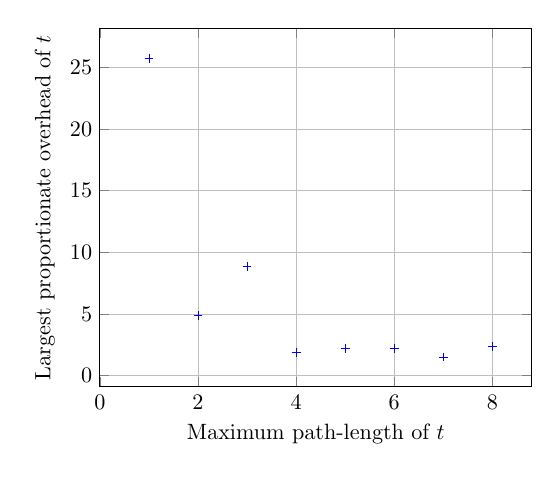
\begin{tikzpicture}[scale=0.8]
    \begin{axis}[
            ylabel=Largest proportionate overhead of $\rg{t}$,
            xlabel=Maximum path-length of $\rg{t}$,
            grid=major,
            xmin=0
           ]
       \addplot[mark=+,only marks,blue] plot coordinates{
            (1,25.7433) (2,4.8584) (3,8.8644) (4,1.876) (5,2.228) (6,2.176) (7,1.51) (8,2.39)
        };    % largestoverheadproportion-pathlength.csv
    \end{axis}
    \end{tikzpicture}
    \caption{Varying \textit{largest} observed overhead \textit{proportion} with maximum path-length.}
    \label{fig:pathlength-largestproportionateoverhead}
\end{subfigure}
\caption{Relationships between $\rg{t}$'s audience overhead properties and its maximum path-length $\forall \, t \in T'$, where $T'$ is the set of analysed Tweets}
\label{fig:4_overhead}
\end{figure}

The power of the retweet phenomeon in terms of how it affects the potential audience reach of a particular Tweet is discussed in further detail by \citet{kwak10}, in which they find that a retweeted Tweet of sufficient interest can reach a very large number of users even if the original author has only a few followers. The same paper more specifically mentions that the audience size of a retweeted Tweet reaches, on average, at least 1,000 users, no matter the number of followers of the original author. This result agrees with the results in Figure \ref{fig:4_overhead}(\subref{fig:pathlength-audience}) in that even Tweets with a short maximum path-length still, on average, have a relatively large audience size.


\subsection{Retweet Groups on the Social Graph}
\label{section:retweets_graph}
Now that an understanding has been achieved in the behaviours and properties of retweets and retweet groups, it is important that the nature of the social ties between users in groups is studied. This will provide a grounding for the research in the following chapter, in which the social structure and its role in facilitating propagation, are discussed in more detail.

It has already been mentioned that the probability of a retweeting author following the original author in unit-length retweet chains was found to be around 90\%. However, in retweet groups with longer chains, a decrease in the likelihood of the final retweeter (the user at the bottom of the retweet tree) following the original author was observed. Indeed, on average across all retweet groups, the final retweeter in the longest chain follows the \textit{previous} retweeter in around 67\% of cases. The final retweeter of a retweet chain is defined as the author of the leaf node of the chain.

%\begin{figure}[h]
%\centering
%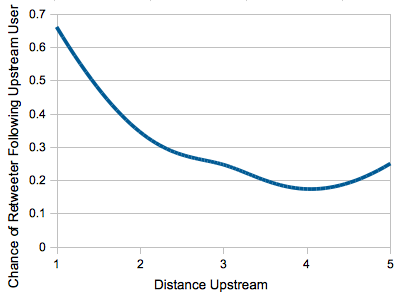
\includegraphics[scale=0.6]{3.Chapter1/Media/following-possibility.png} 
%\caption{\textit{Relationship between the chance of followship between the final retweeter and original author in groups and varying maximum path-length}}
%\label{fig:followingchance_pathlength}
%\end{figure}

It is interesting that this value should be about 20\% lower than in unit-length maximum path-length groups, and it suggests that users have a greater chance of `stumbling over' retweets found on non-friends' timelines whilst browsing through other users. Since it has been shown that with an increase in maximum path-length an increase in the audience size is also observed, then this demonstrates the increased chance of discovery of the Tweet through users searching through others' profiles. In cases where the maximum path-length of $\rg{t}$ is equal to one, then the audience size is far smaller and thus there is a lower chance of users who aren't followers of $\aut{t}{O}$ or $\left\{\aut{r}{R} \forall r \in \rt{t}\right\}$ finding the Tweet.

\begin{figure}[h]
\centering
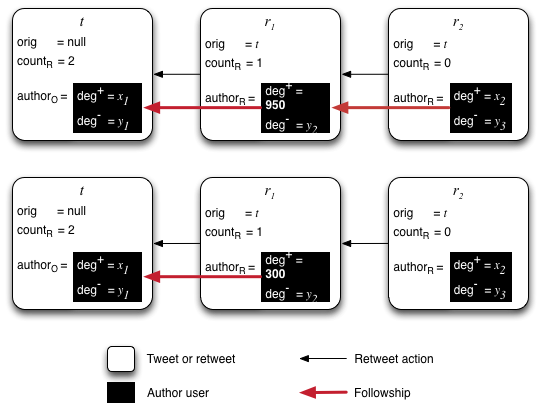
\includegraphics[scale=0.7]{3.Chapter1/Media/final_following_upstream.png} 
\caption{Effect of the final retweeter following the upstream user on the follower count of the upstream user}
\label{fig:final_following_upstream}
\end{figure}

In addition, there is some evidence of user influence playing a role in the analyses of these data. In particular, in the 67\% of retweet groups in which the final retweeter \textit{does} follow the author of the retweet (or original Tweet) directly `upstream', the latter user has, on average, around 950 followers. Inversely, in the remaining 33\% of groups (in which the author of the final retweet does \textit{not} follow the preceding author), the preceding author has an average of 600 followers. This is illustrated by an example in Figure \ref{fig:final_following_upstream} and it implies that there is a significant difference in the retweet potential with varying author influence levels.

\begin{figure}[h]
\centering
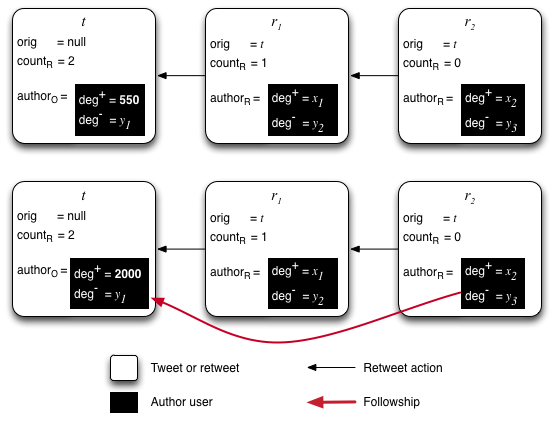
\includegraphics[scale=0.7]{3.Chapter1/Media/final_following_original.png} 
\caption{Effect of the final retweeter following the original author on the follower count of the original author}
\label{fig:final_following_original}
\end{figure}

This is further accentuated when one studies the follower connections of $\aut{t}{O}$ in groups where the maximum path-length is greater than one. Whilst it was found earlier that the likelihood of a $\aut{r}{R}$ following $\aut{t}{O}$ is around 40\%, the average follower count of $\aut{t}{O}$ has a four-fold increase (from about 550 to 2,000) when he/she is also followed by the final retweeter. Figure \ref{fig:final_following_original} demonstrates an example of this in a retweet chain of two retweets; that when the author of $r_3$ follows the author of $t$, then $\foc{\aut{t}{O}}$ is significantly greater. 

In fact, in groups of \textit{all} maximum path-lengths, $\aut{t}{O}$ had a consistently higher follower count when followed also by the final retweeter of $\rg{t}$ than when not followed.

This particular behaviour also helps illustrate that a user is more likely to be retweeted when s/he has more followers - in this case, having four times the follower count increases the correlation dramatically (40\% to 90\%). The follower count can, therefore, be directly related in this way to the discussions of user influence by \citet{cha10}, and also of users using retweeted Tweets to passively `advertise' themselves.

\begin{figure}[h]
\centering
    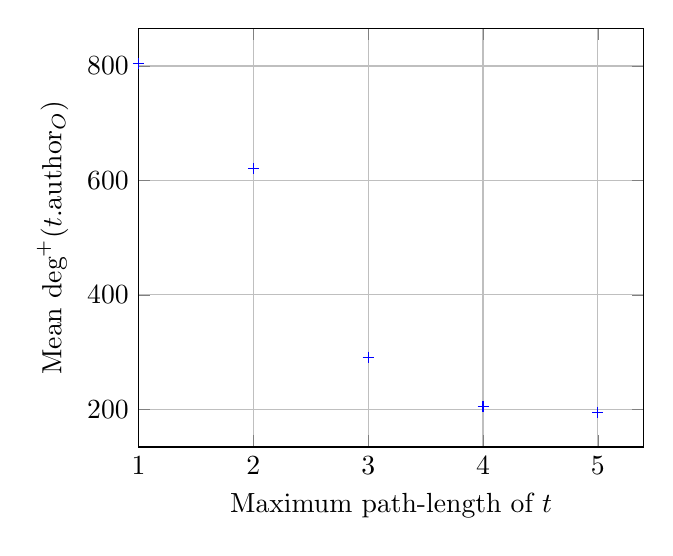
\begin{tikzpicture}
    \begin{axis}[
            ylabel=Mean $\textrm{deg}^+(t.\textrm{author}_O$),
            xlabel=Maximum path-length of $\rg{t}$,
            grid=major,
            xmin=1,
            width=8cm]
       \addplot[mark=+,only marks,blue] plot coordinates{
            (1,805) (2,621) (3,291) (4,205) (5,195)
        };    
    \end{axis}
    \end{tikzpicture}
    \caption{Analysis of variance in $\foc{\aut{t}{O}}$ as $\rg{t}$'s maximum path-length increases}
\label{fig:originalfollowers-pathlength}
\end{figure}


%\begin{figure}[h]
%\centering
%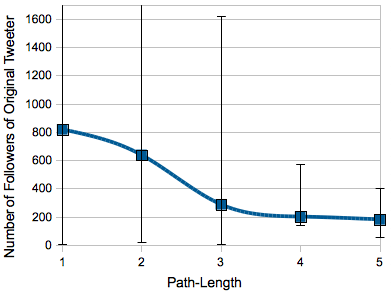
\includegraphics[scale=0.6]{3.Chapter1/Media/originalfollowers-pathlength-distribution.png} 
%\caption{\textit{Relationship between number of followers (and respective distribution) of the original tweeter as the path-length increases}}
%\label{fig:originalfollowers-pathlength}
%\end{figure}

Strangely, Figure \ref{fig:following-possibility} illustrates how increases in maximum path-length of retweet groups caused the follower count of the original author to diminish, indicating further penetrative depth of propagation when the original author has \textit{fewer} followers. The collected retweet groups that contained longer retweet chains often also contained retweet chains that were much shorter. For example, a group containing chains with path-lengths of five, or more, are also likely to contain many more chains with path-lengths of one and two (as is implied in the distribution in Figure \ref{fig:pathlength-distribution}). There are, therefore, various possible explanations for this property, including the argument that users with many followers are generally likely to be part of a large community of users, from which retweets are not transmitted. Users that are part of several communities, and are therefore less involved with any given one, may find that their Tweets have the potential to be retweeted a further distance.

Additionally, and more interestingly, it is possible that users possess some awareness of their local networks and the users within them. A user, who is part of a large community with lots of obvious follower overlaps occurring between the members, may decide \textit{not} to retweet a particular Tweet if he/she feels that many of his/her own followers may be shared with the author and that they might have therefore already seen the Tweet.

A final analysis on the social ties between users in retweet chains is carried out on the followship pattern of authors throughout the chain. Let $h$ be the number of hops (or edges in the retweet tree) between the original author and a retweeter in a retweet chain. It was illustrated in earlier sections that, when $h = 1$, the likelihood of a retweeter following the original author is around 67\%. However, as $h$ is increased, then the followship likelihood mostly consistently decreases. 

Let $\aut{r_h}{R}$ be the author of the retweet $h$ hops from $t$ in $\rg{t}$'s retweet tree. Figure \ref{fig:following-possibility} illustrates how longer retweet chains do indeed increase both the likelihood of the Tweet reaching further through the social structure and the chance of achieving a smaller proportionate overhead.

Further to this, of the 67\% of retweeters who \textit{do} follow the original author when $h = 1$, only 19\% follow also the upstream author at $h = 2$. In these cases, the latter has an observed average of around 3,000 followers. In the 81\% of cases when the user at $h = 2$ \textit{isn't} also followed, then the upstream author has a much lower average follower count of about 520.

\begin{figure}[h]
\centering
    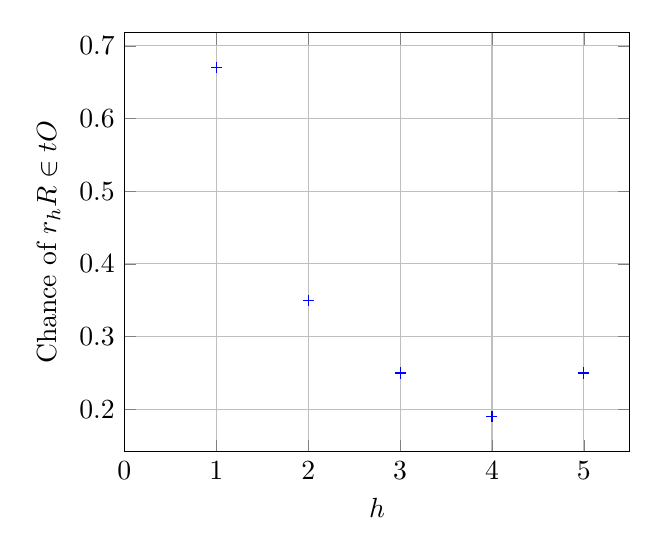
\begin{tikzpicture}
    \begin{axis}[
            ylabel=Chance of $\aut{r_h}{R} \in \fos{\aut{t}{O}}$,
            xlabel=$h$,
            grid=major,
            xmin=0,
            width=8cm]
       \addplot[mark=+,only marks,blue] plot coordinates{
            (1,0.67) (2,0.35) (3,0.25) (4,0.19) (5,0.25)
        };    
    \end{axis}
    \end{tikzpicture}
    \caption{Relationship between the likelihood of $\aut{r_h}{R} \in \aut{t}{O}$ (where $r \in \rt{t}$) and increases in `distance' between $r$ and $t$ given by $h$}
\label{fig:following-possibility}
\end{figure}


%\begin{figure}[h]
%\centering
%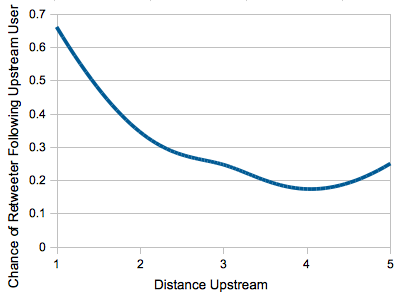
\includegraphics[scale=0.55]{3.Chapter1/Media/following-possibility.png} 
%\caption{\textit{Proportion of final retweeters following upstream users at varying distances along the chain.}}
%\label{fig:following-possibility}
%\end{figure}

It is, therefore, sensible to assume from these analyses that Tweets are forwarded more between groups of less-connected users, highlighting the notions of social network awareness and of community-hopping. If retweets were usually circulated around more closely-knit communities of users, then the followship likelihoods would be generally greater, more uniform, and consistent throughout the retweet chain. Users would have as much of a chance of following their immediate upstream neighbour author in the retweet chain as they would an author further upstream.

As mentioned near the start of this chapter, the author of the original Tweet should be cited by the \texttt{RT @<username>} sequence observed \textit{closest} to the retweet body, where the \texttt{<username>} is the username of the original author user. Rather than specifically looking for the author's Tweet appearing in this location, Tweets were examined to check for the existence of the author's username being mentioned \textit{anywhere} in the Tweet content, and was found to exist in about 68\% of Tweets.

This frequency did not vary with any consistent correlation upon changes to the maximum path-length or retweet group size, and so it is assumed that users do feel the need to credit the original author more so than not. 

 
\subsection{The Temporal Properties of Retweets}
The final set of analyses in this chapter relate to time's influence on retweet propagation. This provides insights into how quickly information can spread and, when combined with the knowledge of the social structure and audience, how this can relate to the rate of information dissemination and consumption.

%\begin{figure}[h]
%\centering
%    \begin{tikzpicture}
%    \begin{axis}[
%            ylabel=Time elapsement (secs.),
%            xlabel=Maximum path-length of $\rg{t}$,
%            grid=major,
%            xmin=1,
%            width=8cm]
%       \addplot[mark=+,blue] plot coordinates{
%            (1,21766) (2,33466) (3,53582) (4,80658) (5,41600) (6,31360) (7,23989) (8,63102) (9,133611) 
%        };    
%    \end{axis}
%    \end{tikzpicture}
%    \caption{Comparison between the average time elapsement from $t$ to the final $r \in 
%\rt{t}$ and the maximum path-length of $\rg{t} \forall t \in T'$, where $T'$ is the set of analysed Tweets}
%\label{fig:timedelay-pathlength}
%\end{figure}

%\begin{figure}[h]
%\centering
%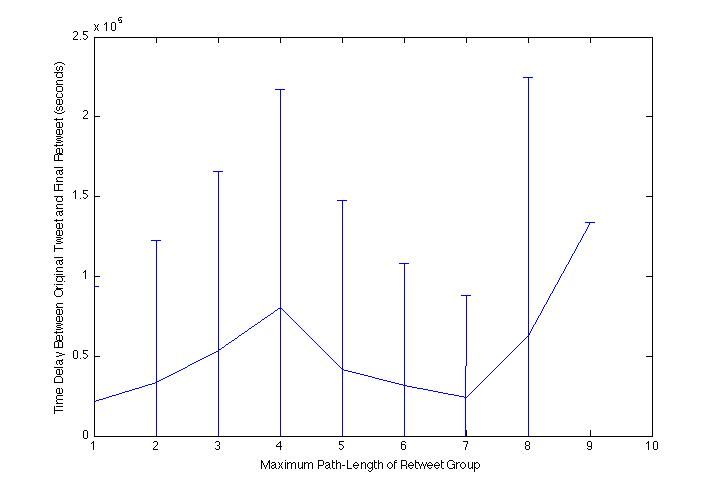
\includegraphics[scale=0.35]{3.Chapter1/Media/pathlength-timedelay.jpg} 
%\caption{\textit{Average time (in seconds) between first post and final retweet of a retweet group varying with the group's maximum path-length}}
%\label{fig:timedelay-pathlength}
%\end{figure}

Generally, it was found that the elapsed time between the original Tweet and the final retweet in retweet groups increased with the groups' maximum path-lengths, indicating that if there are more hops for a Tweet to travel down between users then it takes longer to do so. However, this correlation is only really applicable to shorter retweet chains, which more uniformly increase in elapsed time with increases in maximum path-length in a linear fashion roughly proportional to $ v=\frac{s}{t} $, where the distance, \textit{s}, is the hypothetical distance given by the number of hops between users, thus indicating that the speed, $v$, of propagation remains relatively constant. 

Retweet groups exhibiting longer maximum path-lengths are less consistent in terms of the groups' propagation speeds. Whilst this is likely attributed to smaller samples, there are conflicting arguments for patterns observed in this propagation speed, which rely on various intervening factors. 

As mentioned, the time taken for a Tweet to reach a specific path-length could be a function of the path-length itself, where as the path-length increases, then so does the time taken for the Tweet to be retweeted to the end of the chain. Inversely, Tweets that are especially popular, possibly as a result of being particularly topical (such as in the disaster cases mentioned in the Introduction), may be retweeted more quickly by users so that the information is spread more quickly. In these cases, retweet groups with longer retweet chains may complete their trees more quickly than those groups with much shallower retweet trees.

Similarly, user influence could play a role in dissemination speed; if a Tweet is retweeted by a user with many followers, then there is an increased likelihood of propagation through this user. Whilst this could, in addition to the previous argument, cause longer retweet trees to be completed more quickly than groups with shorter trees, it could also facilitate `faster branches', in which particular long branches grow faster and reach their leaves more quickly than shorter ones in the same retweet tree, if the other branches consist of less-influential authors and retweeters.

There is not enough evidence provided in this analysis to make any inferences towards a generic pattern of retweet group growth speed, and it is believed that this growth is governed by many more factors than the Tweet itself or the social structure alone. As such, there is no predefined rule for predicting the spread of dissemination in this way, since the retweet path is an unknown feature, with too many variables and conflicting arguments.

The temporality of retweets has been the focus of some researchers, including \citet{kwak10}, who also used retweet trees as an illustration of the propagation pattern produced by Tweets. They found that, generally, half of all retweet action on a Tweet occurs \textit{within an hour} of the Tweet being posted, and that by the end of the first day, 75\% of all retweets of the Tweet will have been carried out. The authors also conducted an analysis on the elapsed time of a Tweet's travel between hops as it is retweeted. Although they observe a `flatter' time initially, indicating that Tweets travelling over the first few hops are retweeted almost concurrently, they also found there to be a general incline in time taken for retweets to occur over the shorter path-lengths. After this point, the time taken becomes more `noisy'. 

An interesting notion that is not directly addressed in this thesis is that the time a particular Tweet is authored may have some effect on its propagation speed. Just as `prime-time' television achieves higher audience ratings as it is at a time of the day when many people are at home and relaxing, Twitter may also exhibit a prime-time window in which its users are more active. For example, if a user posts a Tweet at a time when many of his/her followers are asleep, then the immediate audience size of the Tweet can be significantly reduced.

If there are fewer initial users viewing the Tweet, then the likelihood of retweet, as a function of this, is also reduced. This could have an effect on the perceived popularity of the Tweet, although since, by definition, there are fewer active users on Twitter at this time, then the number of Tweets sent during this period will be much smaller. Therefore, this is not taken into account during experimentation in later chapters.


\section{Summary}
In this chapter, a set of initial exploratory analyses have been undertaken into the behaviour of retweets and retweet activity in Twitter, the properties of retweet groups, the relationships between the propagation graph and the social graph, and briefly into the effects of time on Tweet dissemination.

The analyses were found to support and complement the findings of other research in the area, including the notions of message cascading \cite{galuba10} and the relationships of this to the interconnection of users on the social graph through communities \cite{java07}. Trees representing the retweet groups were found to grow in a variety of ways, from those illustrating long retweet chains, indicating a high level of inter-community dissemination, to shorter and wider trees, in which propagation can still be widespread but not as likely to disseminate to other communities.

User influence, in terms of an author's follower count, was observed as being an important factor in facilitating information spread, implying that popular users also produce popular information, since these users are more likely to achieve more retweets.

These inferences have helped to describe the multi-dimensional principles of retweet groups in terms of the features governing their spread over the social graph, and the quickness with which many users can be exposed to a Tweet. Although it is important to have an understanding of user psychology, and the thought processes behind the retweet decision, of most interest in this chapter is the analysis of the social structure.


\section{Taking the Investigative Research Further}
Twitter's social structure has been found to have a large effect on Tweet propagation, since it combines the features observed around user influence (in the na{\"i}ve form of a user's follower count) with that of communities and sub-graphs of dense and sparse user interconnections.

In the following chapter, interests are focused on research questions \textbf{RQ3} and \textbf{RQ4}, in which the topological structure of user followships is studied through investigations into the flow of information between users arranged differently on the social graph. This research is conducted in order to develop a method to infer information interestingness, taking into account these information flow properties and user influence. It is clear that different Tweets can have a different level of \textit{quality} in that Tweets that are retweeted have a greater chance of being interesting, but does the way in which the social structure of users is formed also have a `quality' in terms of the propagation characteristics exhibited?
